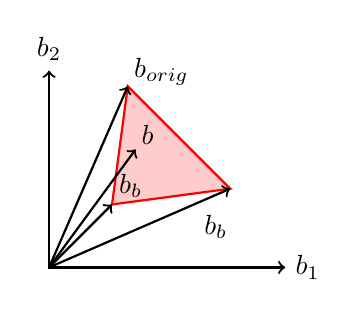
\begin{tikzpicture}
    % Draw axes
	\coordinate (borig) at (1,2.3);
    \coordinate (b_a) at (0.8,0.8);
	\coordinate (b_b) at (2.3,1);
	\coordinate (b) at (1.1,1.5);


    \draw [<->,thick] (0,2.5) node (yaxis) [above] {$b_2$}
        |- (3,0) node (xaxis) [right] {$b_1$};

    \draw[thick,red,fill = red!20] (borig) -- (b_a) -- (b_b) -- cycle;

	\draw[thick,->] (0,0) -- node[anchor=south west,pos = 0.95] {$b_{orig}$} (borig);
    \draw[thick,->] (0,0) -- node[anchor=south west,pos = 0.95] {$b_b$} (b_a);
    \draw[thick,->] (0,0) -- node[anchor=south west,pos = 0.95] {$b$} (b);
	\draw[thick,->] (0,0) -- node[anchor=north west,pos = 0.8,fill=white] {$b_b$} (b_b);

\end{tikzpicture}